\documentclass[a4paper,10pt]{article}
\usepackage{graphicx}
\usepackage[spanish]{babel}
\usepackage[latin1]{inputenc}
\usepackage{a4wide}
\usepackage{amsmath}
\usepackage{amssymb}
\usepackage{graphicx}
\usepackage{eqnarray}
\usepackage{epstopdf}
\usepackage{subfigure}
\usepackage{natbib}
\usepackage{algorithm}
\usepackage{hyperref}

\usepackage{amsfonts}  % For \mathbb
\usepackage{bm}   % command \bm

\usepackage{xcolor}
\usepackage{listings}
\lstset{basicstyle=\ttfamily,
  showstringspaces=false,
  commentstyle=\color{red},
  keywordstyle=\color{blue}
}

\begin{document}

\title{Crazyflie 2.1 - ROS (\texttt{uned\_crazyflie\_ros\_pkg})}
\author{Francisco J. Ma�as-�lvarez}     
\date{\today}
\maketitle
\tableofcontents
\newpage

% -------------------------------------
\section{Introducci�n}
% -------------------------------------
Este repositorio\footnote{Github: \url{https://github.com/FranciscoJManasAlvarez/uned_crazyflie_ros_pkg}} contiene los paquetes de ROS y ficheros de configuraci�n para la teleoperaci�n y simulaci�n del dron crazyflie 2.1 en ROS, Gazebo y Matlab. Se busca obtener una herramienta Hardware-in-the-Loop que sea facilmente escalable y mantenible. A partir de esta herramienta, se pretende integrar estos robots en un sistema distribuido mayor con m�s variedad de robots.

\subsection{Estructura}

\begin{itemize}
\item\textbf{doc.} Contiene un fichero \textit{.tex} que aborda m�s en detalle toda la informaci�n relacionada con el repositorio: esquemas de ROS, b�squedas bibliogr�ficas, enlaces de inter�s, etc.

\item\textbf{scripts.} Contiene aquellos ficheros auxiliares que no forman parte de ning�n paquete de ROS. Por ejemplo, ficheros \textit{.sh} para automatizar procesos repetitivos como la conversi�n de los ficheros \textit{.bag} a txt o los scripts de Matlab para representar datasets.

\item\textbf{submodules.} En este directorio est�n vinculados otros repositorios que se reutilizan, o se toman de base, para tareas ya abordadas por otros usuarios.

\item\textbf{uned\_crazyflie\_config.} Paquete de ROS. Contiene aquellos elementos auxiliares para la configuraci�n del entorno, as� como los \textit{.launch} para la ejecuci�n en bloque de las diferentes estructuras del sistema.

\item\textbf{uned\_crazyflie\_drone.} Paquete de ROS. Comprende los nodos propios desarrollados para la integraci�n de drones en el sistema. Incluye toda la informaci�n asociada para su correcta puesta en marcha.

\item\textbf{uned\_crazyflie\_test.} Paquete de ROS. Paquete en el que se incluyen todos los elementos destinados a realizar comprobaciones en el sistema de forma r�pida. Por ejemplo los nodos \textit{talker} y \textit{listener} que se desarrollan al empezar a usar ROS, que en este caso se usan para comprobar la correcta comunicaci�n entre m�quinas en el sistema distribuido.

\end{itemize}

\subsection{Crazyflie}
TO-DO: Describir detalladamente el dron e incluir enlaces a los diferentes trabajos y videos realizados con �l.

Lorem ipsum dolor sit amet, consectetur adipiscing elit. Proin euismod, erat ultrices hendrerit consequat, ligula nisi semper felis, id euismod ex erat eget diam. Vestibulum ut leo condimentum, ullamcorper orci id, suscipit arcu. Suspendisse suscipit purus tincidunt ex eleifend, sed tristique eros maximus. Donec vitae nisl congue, gravida orci vitae, consectetur sapien. Interdum et malesuada fames ac ante ipsum primis in faucibus. Duis ante orci, blandit rutrum urna in, mollis commodo lorem. Donec blandit, velit sed aliquam auctor, mi nunc lobortis arcu, in imperdiet sapien est vitae libero. Donec tincidunt quam ipsum, vitae rhoncus dolor efficitur id. Proin laoreet, ipsum quis vehicula condimentum, ex ipsum tincidunt est, bibendum iaculis enim est vel risus.

Lorem ipsum dolor sit amet, consectetur adipiscing elit. Proin euismod, erat ultrices hendrerit consequat, ligula nisi semper felis, id euismod ex erat eget diam. Vestibulum ut leo condimentum, ullamcorper orci id, suscipit arcu. Suspendisse suscipit purus tincidunt ex eleifend, sed tristique eros maximus. Donec vitae nisl congue, gravida orci vitae, consectetur sapien. Interdum et malesuada fames ac ante ipsum primis in faucibus. Duis ante orci, blandit rutrum urna in, mollis commodo lorem. Donec blandit, velit sed aliquam auctor, mi nunc lobortis arcu, in imperdiet sapien est vitae libero. Donec tincidunt quam ipsum, vitae rhoncus dolor efficitur id. Proin laoreet, ipsum quis vehicula condimentum, ex ipsum tincidunt est, bibendum iaculis enim est vel risus.

\begin{figure}[ht]
  \centering
    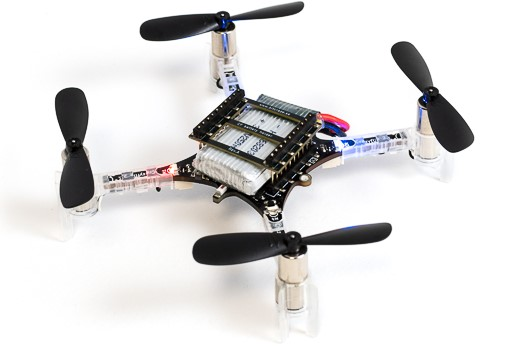
\includegraphics[width=0.63\textwidth]{figs/Crazyflie_2.1.jpg}
  \caption{Crazyflie 2.1.}
  \label{fig:rosgraph}
\end{figure}

\subsection{Proyectos anteriores}
En este apartado se describen los trabajos ya realizados sobre crazyflie que se han consultado y reutilizado parcialmente para la herramienta desarrollada.

\subsubsection*{CrazyS \footnote{Github: \url{https://github.com/gsilano/CrazyS}}}
TO-DO

Lorem ipsum dolor sit amet, consectetur adipiscing elit. Proin euismod, erat ultrices hendrerit consequat, ligula nisi semper felis, id euismod ex erat eget diam. Vestibulum ut leo condimentum, ullamcorper orci id, suscipit arcu. Suspendisse suscipit purus tincidunt ex eleifend, sed tristique eros maximus. Donec vitae nisl congue, gravida orci vitae, consectetur sapien. Interdum et malesuada fames ac ante ipsum primis in faucibus. Duis ante orci, blandit rutrum urna in, mollis commodo lorem. Donec blandit, velit sed aliquam auctor, mi nunc lobortis arcu, in imperdiet sapien est vitae libero. Donec tincidunt quam ipsum, vitae rhoncus dolor efficitur id. Proin laoreet, ipsum quis vehicula condimentum, ex ipsum tincidunt est, bibendum iaculis enim est vel risus.

\subsubsection*{Crazyflie\_ros \footnote{Github: \url{https://github.com/whoenig/crazyflie_ros}}}
TO-DO

Lorem ipsum dolor sit amet, consectetur adipiscing elit. Proin euismod, erat ultrices hendrerit consequat, ligula nisi semper felis, id euismod ex erat eget diam. Vestibulum ut leo condimentum, ullamcorper orci id, suscipit arcu. Suspendisse suscipit purus tincidunt ex eleifend, sed tristique eros maximus. Donec vitae nisl congue, gravida orci vitae, consectetur sapien. Interdum et malesuada fames ac ante ipsum primis in faucibus. Duis ante orci, blandit rutrum urna in, mollis commodo lorem. Donec blandit, velit sed aliquam auctor, mi nunc lobortis arcu, in imperdiet sapien est vitae libero. Donec tincidunt quam ipsum, vitae rhoncus dolor efficitur id. Proin laoreet, ipsum quis vehicula condimentum, ex ipsum tincidunt est, bibendum iaculis enim est vel risus.

% -------------------------------------
\section{Instalaci�n}
% -------------------------------------



% -------------------------------------
\section{Simulador}
% -------------------------------------

% -------------------------------------
\section{Hardware-in-the-Loop}

\subsection{Crazyflie\_ros}
TO-DO
\begin{figure}[ht]
  \centering
    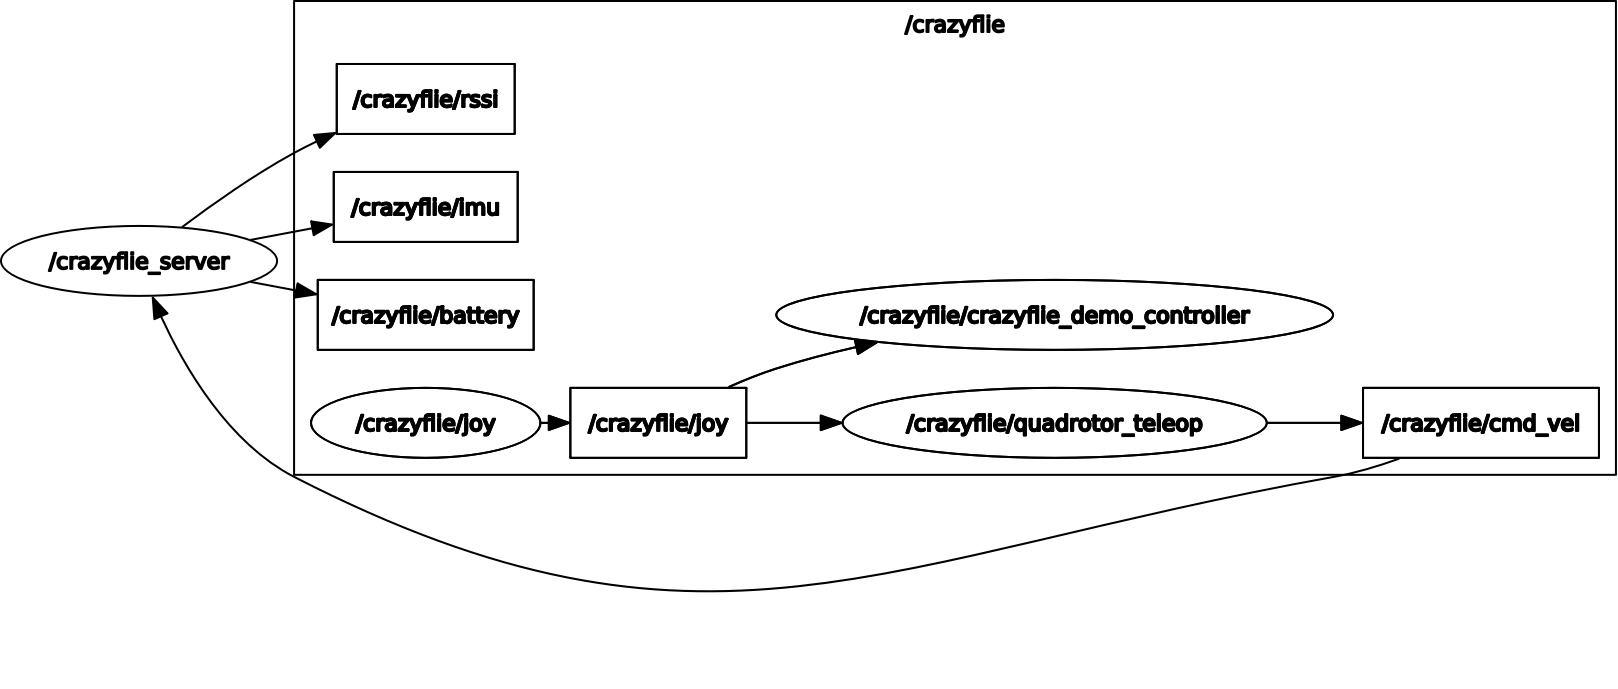
\includegraphics[width=1.0\textwidth]{figs/rosgraph.png}
  \caption{rosgraph.}
  \label{fig:rosgraph}
\end{figure}

%% ---------------------------------------------------------------
%%                         BIBLIOGRAPHY
%% ---------------------------------------------------------------
%\bibliographystyle{plain}
%\bibliography{refs}


\end{document}